%
% File naaclhlt2010.tex
%
% Contact: nasmith@cs.cmu.edu

\documentclass[11pt,letterpaper]{article}
\usepackage{naaclhlt2010}
\usepackage{times}
\usepackage{latexsym}
\usepackage{amsmath}
\usepackage{hyperref}
\usepackage{graphicx}
\DeclareMathOperator*{\argmax}{arg\,max}
\setlength\titlebox{6.5cm}    % Expanding the titlebox

\title{A Network-Assisted Approach to Predicting Passing Distributions}

\author{
  Jade Huang\\
  Stanford University \\
  {\tt jayebird@stanford.edu}}

\date{}

\begin{document}
\maketitle
\begin{abstract}
% What is it that you are trying to solve/achieve and why does it matter?

\end{abstract}

\section{Introduction}

\section{Related Work}
% How does your project relate to previous work. Please give a short summary on each paper you cite and include how it is relevant.

\section{Model}

% This is where you give a detailed description of your primary contribution. It is especially important that this part be clear and well written so that we can fully understand what you did.

Given a team A's past passing distributions, a team B's past passing distributions, the average lineup of team A, and the average lineup of team B, the goal is to predict the edges between players for both team A and team B when team A and team B face each other in a match.

Due to the observation that lineups do not change dramatically for a team between matches, we randomly choose a lineup used by a team during the group stage and hold it as constant as we seek to predict the edges between players.

\subsection{Baseline}

For a baseline model, the average of past passing networks during the group stage is used to predict the passing networks during the round of 16 stage. Thus, during training, for every player to player combination in each team for which there exists a pass, the total number of passes over six games is calculated during the group stage and averaged over the number of games. 

The average values calculated during training are used to predict the number of passes for each team in each game in the round of 16 of the 2014-15 season. For example, if in team X, player 1 passed to player 9 an average of five times during the group stage, this baseline model would predict that player 1 would pass to player 9 five times when playing some team in the round of 16.

This is a naïve baseline that does not take into account the specific opponent during each of the past games during the group stage, but merely generalizes, ignoring any idiosyncrasies which may arise when facing a higher ranked or lower ranked opponent. 

\section{Algorithm}

To build upon the baseline, a linear regression model was constructed to include features that are indicative of the amount of passes between two players and which would learn weights which would correspond how descriptive a feature is in relation to the amount of passes between two players.

\subsection{Features}
With guidance from Tim Althoff, I postulated the following are key ingredients leading to how often two certain players pass:

\begin{itemize}
\item Average number of past passes between two players. This is a continuous value that is pre-computed before the process of training and learning weights. As with the baseline, the average of all passes between two players for each player for each team over all "past" games, where the notion of past is experimented with later on, is taken.
\item Whether two players are of the same position. This is a boolean value which fires $1$ if the condition is true and $0$ otherwise. The motivation for this feature is that based on analyzing the data, certain positions pass to each other very often, such as from defender to midfielder, while others never pass to each other, such as goalkeeper to goalkeeper.

% bar graph
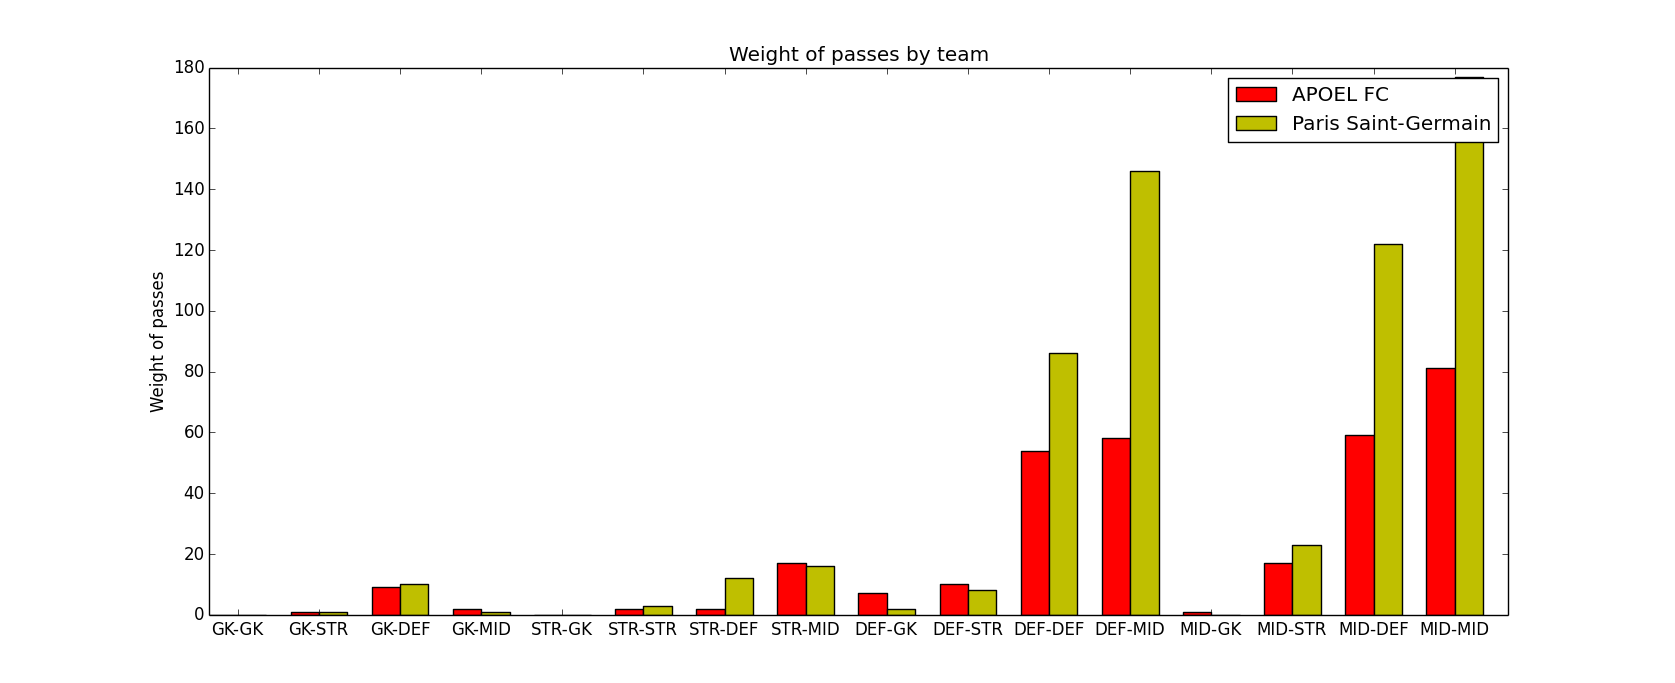
\includegraphics[scale=0.20]{APOEL_FC-Paris_Saint-Germain.png}

\item Whether two players have different positions. This feature also is a boolean value which is the negation of the previously mentioned feature. The motivation for this feature, in addition to the motion for the previously mentioned feature, is that perhaps the difference in position could be additionally indicative than the sameness in position.
\item Whether team A's rank is higher than team B's rank. This feature is a boolean value which fires $1$ if team A's rank is higher than team B's rank, and $0$ otherwise. The motivation is that perhaps players may pass more or less depending on whether the opponent team is ranked higher or worse. 
\item Whether team A has won against a "similar" team as team B in the past. In every subsequent stage, teams play teams that they haven't played in previous stages--thus there is no previously existing data stored for team combinations at testing time. Thus, it may be helpful to find a team C that is similar to a team B in team A's play history and use the outcome of that match in determining if team A has a good chance of winning against team B.
\item Whether team A's average pass completion rate is higher than team B's pass completion rate. This is a boolean value which fires $1$ if team A's average pass completion rate is higher than team B's pass completion rate, and $0$ otherwise. The average is taken of pass completion rates across past games ignoring specific opponents. In analyzing the data, a trend was observed where 63.5\% of the time the team with a higher pass completion rate was also the team that lost the match. 
\item Whether volume of passes for team A is higher on average than the volume of passes for team B. This is a boolean value which fires $1$ if team A's average passing volume  is higher than team B's average passing volume, and $0$ otherwise. The average is taken of passing volumes across past games ignoring specific opponents. In analyzing the data, a trend was observed where 62.5\% of the time the team with a higher volume of passes was also the team that lost the match.
\item Average number of passes between two positions. This is a continuous value representing the average number of passes between two positions on a team. The motivation is that perhaps on a team, two given positions generally pass to each other some similar amount across all games.
\end{itemize}

\subsection{Data}
Data used includes team passing distributions and tactical lineups provided by the UEFA Champions League press kits for the Group, Round of 16, Quarter-finals, and Semifinal stages of the \href{http://www.uefa.org/mediaservices/presskits/uefachampionsleague/season=2015/index.html}{2014-15 season}. 

Passing distributions included number of passes completed between all players as well as the total number of passes completed and pass for each of the 32 teams in the Group stage, each of the 16 teams in the Round of 16 stage, each of the 8 games in the Quarter-finals stage, and each of the 4 games in the Semi-finals stage. Using Python and bash scripts, the number of passes between players were parsed into a $csv$ format including the source player of the pass, the destination player of the pass, and the weight of the pass which represents the number of passes completed from the source player to the destination player.

In addition, the positions of each squad were also acquired from the press kits provided by the UEFA using the Squad List section. I copied each squad list into an Excel spreadsheet, which I parsed into a $csv$ format using a Python script.

The rankings of each team were copied into a $csv$ format by hand for relevant teams in the 2014-15 season from the 2013-14 season from \href{http://www.uefa.com/memberassociations/uefarankings/club/season=2015/index.html}{UEFA rankings for club competitions}.
\section{Results}

% How do you evaluate your solution to whatever empirical, algorithmic or theoretical question you have addressed and what do these evaluation methods tell you about your solution? It is not so important how well your method performs but rather how interesting and clever your experiments and analysis are.

% We are interested in seeing a clear and conclusive set of experiments which successfully evaluate the problem you set out to solve. Make sure to interpret the results and talk about what we can conclude and learn from your evaluations. Even if you have a theoretical project you should have something here to demonstrate the validity or value of your project (for example, proofs or runtime analysis).
\subsection{Evaluation}

I utilized the squared loss to capture the accuracy of a prediction of number of passes between two players in comparison to the actual number of passes between two players. The score $\phi(x) \cdot \mathbf{w}$ is considered the prediction while $y$ represents the actual number of passes.

\begin{align*}
Loss_{squared} &= ({\tt predicted} - {\tt actual})^2 \\
&= (\phi(x) \cdot \mathbf{w} - y)^2
\end{align*}

To evaluate my model as a whole, I took the average of the loss over all passes between players. In the below equation, $T$ represents the total number of passes between players over all teams and games during the round of 16 stage.

\begin{equation}
Loss_{model} = \frac{1}{T} \sum_{i = 0}^{i = T} (\phi(x) \cdot \mathbf{w} - y)^2
\end{equation}

\subsection{Baseline}
The baseline model has an average loss of $15$, which was calculated by summing up the individual loss for each player to player pass and dividing by the total number of passes during the round of 16 stage. 

For the predicted number of passes to differ from the actual number of passes by $15$ on average can be explained by the generalization made when averaging over all past passes. In addition, the games played during the Round of 16 have teams playing other teams that they did not play during the Group stage. Thus, the baseline is utilizing data that while generalizes how much players will pass to each other on average, fails to capture any changes in style a team may implement in the face of different opponents. 

\subsection{Linear Regression Model}
\subsubsection{Using shared model weights}
I first experimented with using one set of weights for the model, disregarding differences in teams.

No matter how many iterations are run through the six matchdays in order of increasing matchday in the group stage, the following results arise,

\begin{tabular} {|c|c|}
\hline Feature Added & Average Loss \\ \hline
Average Passing Networks & 14.3420 \\ \hline
+ is Same Position & 13.6145 \\ \hline
+ is Different Position & 11.7954 \\ \hline
+ has Higher Rank & 11.8618 \\ \hline
+ Won Against Similar Team & 12.0889 \\ \hline
+ Average Passes Betw. Positions & 12.1446 \\ \hline
+ has Higher Average Pass Volume & 12.2467 \\ \hline
+ has Higher Pass Completion \% & 12.5603 \\ \hline
\end{tabular} 

At first, I was perplexed that even if I ran two iterations or ten iterations I still arrived at the same weights. The weights were being updated with every example, but despite initializing at zero or at the final weight, the weights settled into the exact same value. It appeared to be a bad case of overfitting.

As an experiment, I shuffled the order of matchdays and found that the weights varied with each iteration, but upon test time, increasing the number of iterations didn't necessarily mean that the average loss decreased during testing time. Realistically, it does not make sense to shuffle the matchdays, as the matchdays occur in chronological order and a sort of history is accumulated.

For a more realistic experiment, I shuffled the order of games in each matchday each iteration. As with the experiment of shuffling the order of matchdays, it became evident that resulting weight is dependent on the order of the games and when using even just one feature, the resulting average loss from the resulting weight can vary from $14.512204$ to $18.511490$. By doing away with overfitting, I was left with a large amount of variance. Again, increasing the number of iterations during training time didn't necessarily mean a lower average loss during testing time.

While overall adding in additional features with a linear regression model that learned weights decreased the average loss from the baseline by 21.36\% at best, I experienced issues of overfitting when iterating through the data in a chronological order and, on the other spectrum, issues of variance when shuffling the data during training time.

\subsection{Using team-specific model weights}
% TODO
\section{Problems Encountered}


\section{Future Direction}


\begin{thebibliography}{}
% TODO: cite relevant papers

\bibitem[\protect\citename{Murty \bgroup et al.\egroup }2011]{Murty:11}
Narasimha Murty, M., Susheela Devi, V.
\newblock 2011.
\newblock Pattern Recognition: An Algorithmic Approach.

\bibitem[\protect\citename{Marchetti-Bowick \bgroup et al.\egroup }2012]{Marchetti-Bowick:12}
Micol Marchetti-Bowick and Nathanael Chambers.
\newblock 2012.
\newblock Learning for Microblogs with Distant Supervision: Political Forecasting with Twitter.
\newblock {\em In Proceedings of the European Association for Computational Linguistics},
\newblock Avignon, France.

\bibitem[\protect\citename{Go \bgroup et al.\egroup }2009]{Go:09}
Alec Go, Richa Bhayani, and Lei Huang.
\newblock 2009.
\newblock Twitter Sentiment Classification using Distant Supervision.

\bibitem[\protect\citename{Jurafsky \bgroup et al.\egroup }2008]{Jurafsky:08}
Jurafsky, Daniel and Martin, James H.
\newblock 2008.
\newblock {\em Speech and Language Processing},

\end{thebibliography}

\end{document}
